% Toolbar icon: renumber — an irregularly spaced run of tick marks above an
% arrow, and an evenly spaced run below it: "close the gaps in the id space".
% Deliberately a different drawing from reorder.tex (three bars + a sort arrow),
% because the two forms sit next to each other in the Mesh Modification sidebar
% and mean genuinely different things: reorder changes storage order, renumber
% changes the ids themselves.
\documentclass[tikz,border=2mm]{standalone}
\usetikzlibrary{arrows.meta,calc,shapes.geometric}
\begin{document}
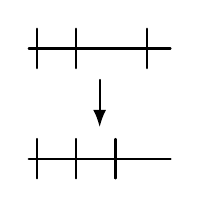
\begin{tikzpicture}[line width=1.3pt, line cap=round, line join=round, x=1mm,y=1mm]
  % Baseline with gappy ticks.
  \draw[thick] (-9,7) -- (9,7);
  \draw[thick] (-8,4.5) -- (-8,9.5);
  \draw[thick] (-3,4.5) -- (-3,9.5);
  \draw[thick] (6,4.5) -- (6,9.5);
  % Downward arrow: the compaction.
  \draw[thick,-{Latex[length=2.2mm]}] (0,3) -- (0,-3);
  % Baseline with evenly spaced ticks.
  \draw[thick] (-9,-7) -- (9,-7);
  \draw[thick] (-8,-9.5) -- (-8,-4.5);
  \draw[thick] (-3,-9.5) -- (-3,-4.5);
  \draw[thick] (2,-9.5) -- (2,-4.5);
\end{tikzpicture}
\end{document}
